\usetikzlibrary{arrows.meta,shapes.geometric}
\tikzset{
    >=Latex,
    resource/.style={draw,rectangle,very thick,align=center},
    resource m/.style={draw,rectangle,very thick,align=center,row sep=2mm},
    resource circle/.style={circle,fill=black,inner sep=0mm,minimum width=2.5mm},
    thread/.style={draw,ellipse,very thick,align=center},
    dependency/.style={draw,ultra thick,->},
    dependency future/.style={dependency,dotted},
    dependency reason/.style={align=center},
}


\section{deadlock examples}

\subsection{a one-way bridge}
\begin{frame}{the one-way bridge}
\begin{tikzpicture}
\tikzset{
    bridge line/.style={ultra thick},
    road divide/.style={very thick,loosely dashed},
    old car black/.pic={
        \node at (0,-0.25) {
\includegraphics[width=1.25cm,angle=-90,origin=c]{../deadlock/Car_icon_top.pdf}};
    },
    old car black opposite/.pic={
        \node at (0,-0.25) {
\includegraphics[width=1.25cm,angle=90,origin=c]{../deadlock/Car_icon_top.pdf}};
    },
    old car black opposite rot/.pic={
        \node at (0,-0.25) {
\includegraphics[width=1.25cm,angle=85,origin=c]{../deadlock/Car_icon_top.pdf}};
    },
    old car red/.pic={
        \node at (0,-0.25) {
\includegraphics[width=1.25cm,angle=-90,origin=c]{../deadlock/Car_red.pdf}};
    },
    old car red rot/.pic={
        \node at (0,-0.25) {
\includegraphics[width=1.25cm,angle=-100,origin=c]{../deadlock/Car_red.pdf}};
    },
    car black opposite/.pic={
        \node at (0,-0.25) {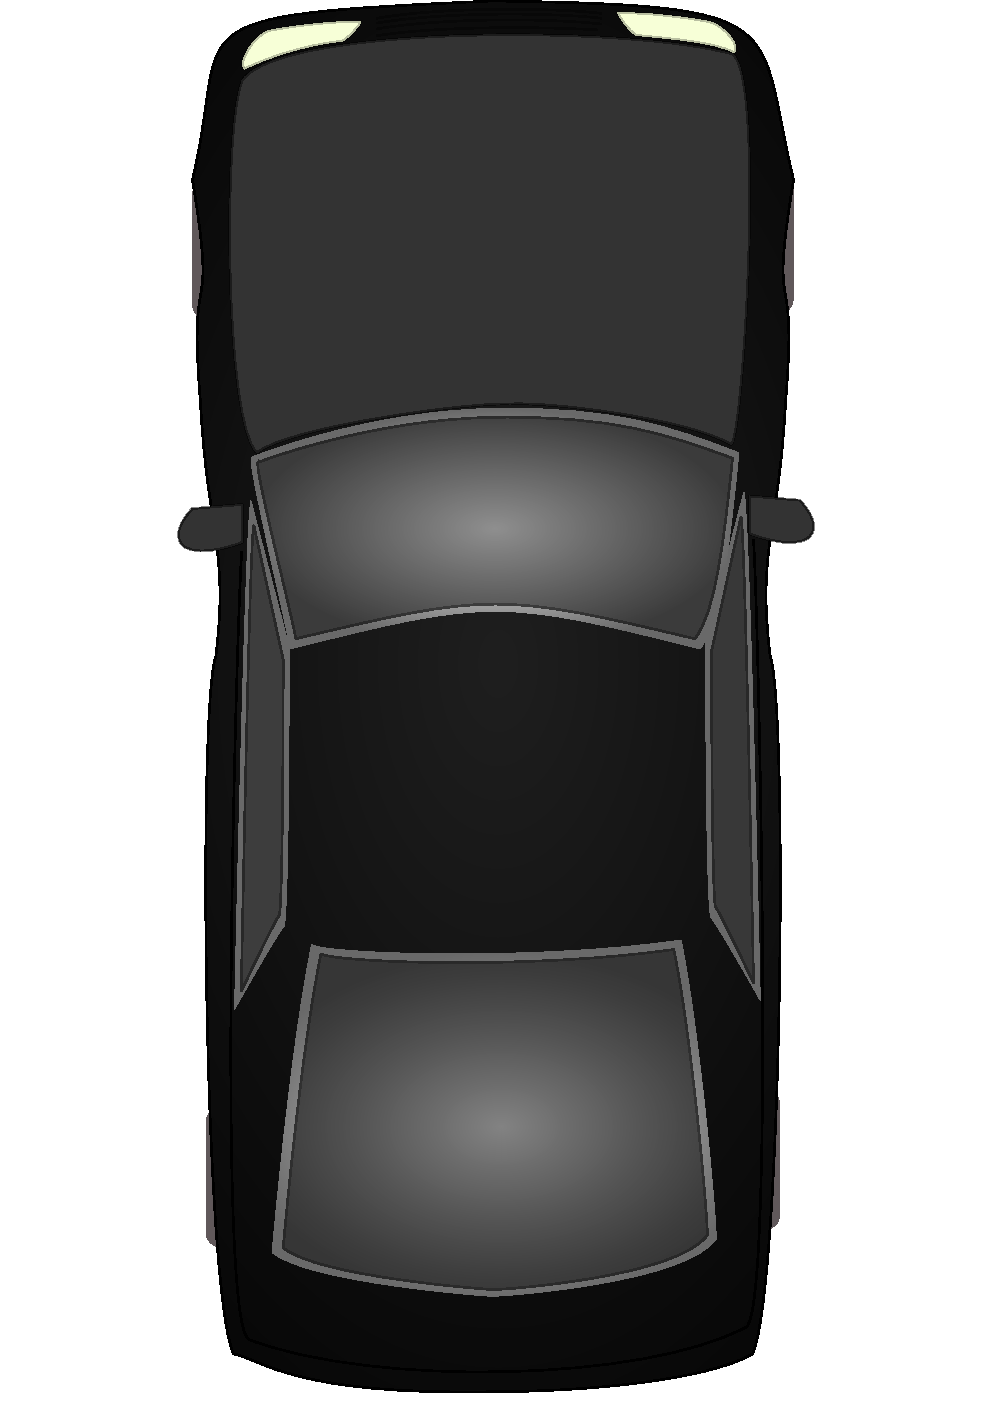
\includegraphics[width=2cm,angle=90,origin=c]{../deadlock/car-black.pdf}};
    },
    car black opposite rot/.pic={
        \node at (0,-0.25) {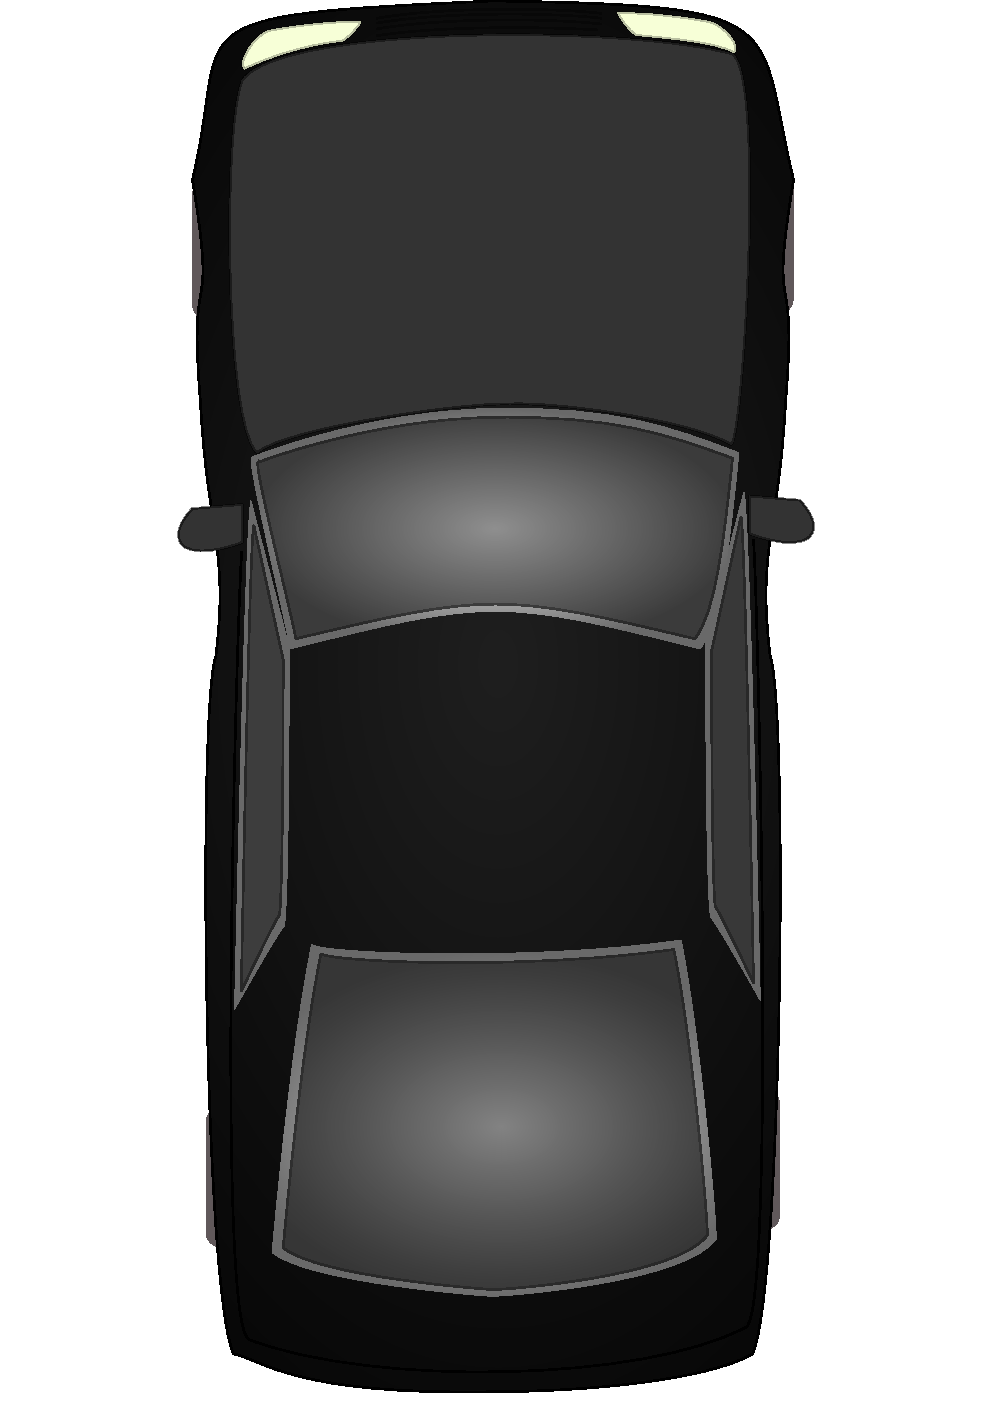
\includegraphics[width=2cm,angle=85,origin=c]{../deadlock/car-black.pdf}};
    },
    car yellow/.pic={
        \node at (0,-0.25) {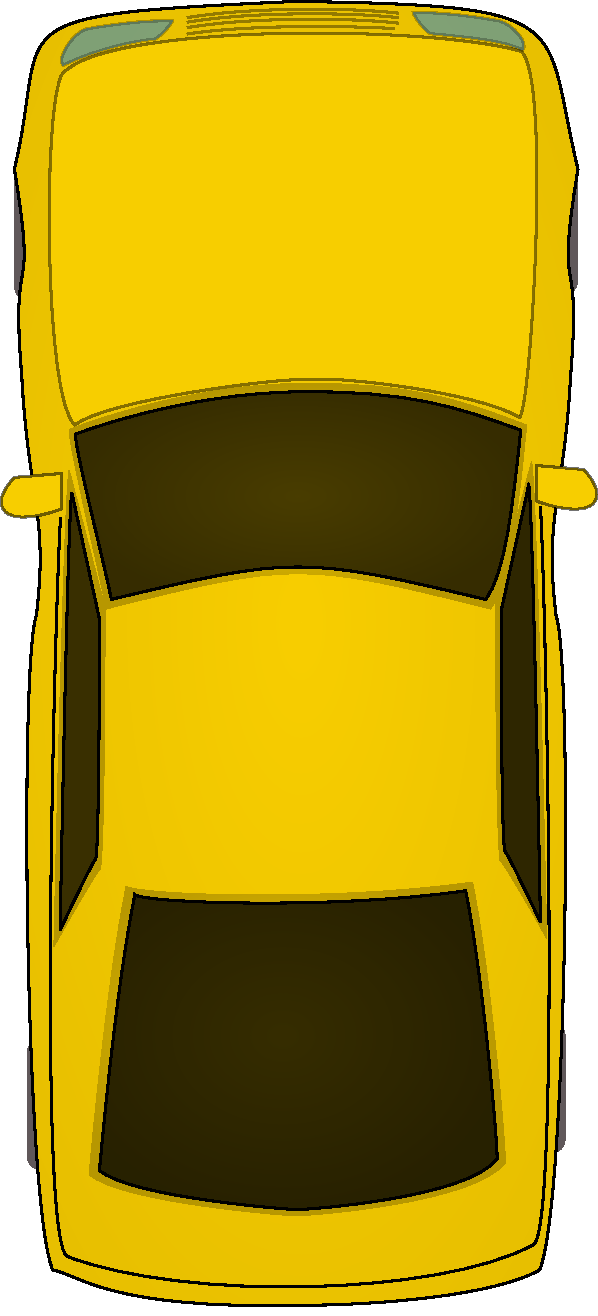
\includegraphics[width=1.25cm,angle=-90,origin=c]{../deadlock/car-yellow.pdf}};
    },
    car yellow rot/.pic={
        \node at (0,-0.25) {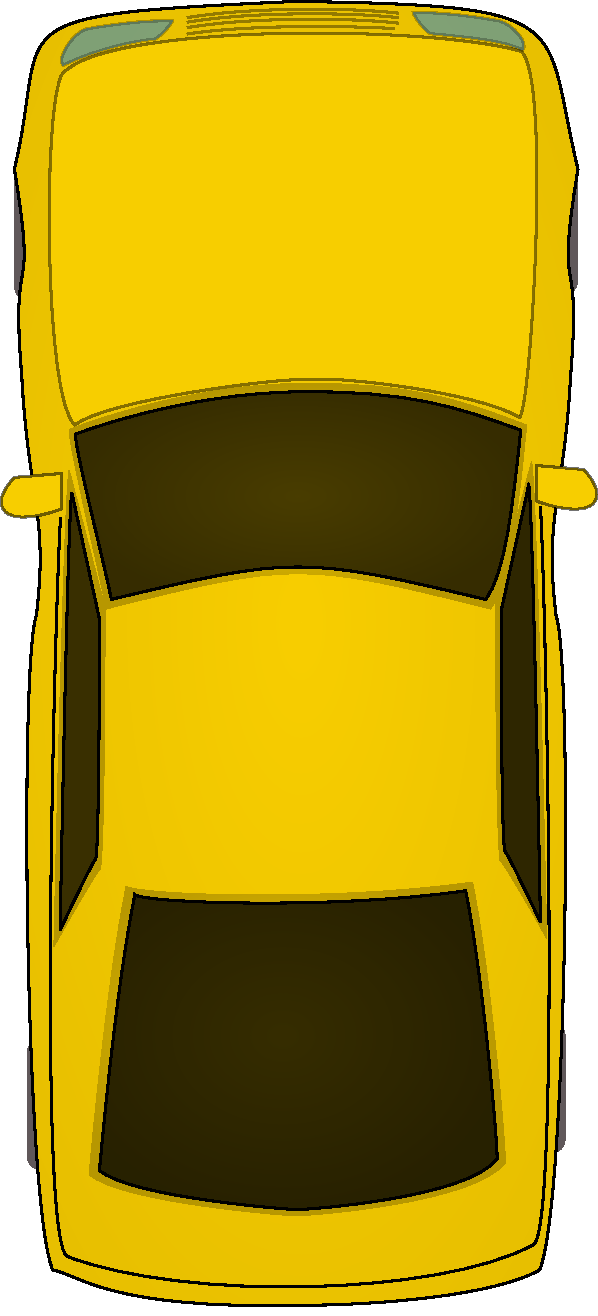
\includegraphics[width=1.25cm,angle=-100,origin=c]{../deadlock/car-yellow.pdf}};
    },
}
\draw[bridge line] (-4.5, -1) -- (-1, -1) -- (1, 0) -- (5, 0) -- (7, -1) -- (10.5, -1);
\draw[bridge line] (-4.5, 3) -- (-1, 3) -- (1, 2) -- (5, 2) -- (7, 3) -- (10.5, 3);
\draw[road divide] (-4.5, 1) -- (-1.5, 1);
\draw[road divide] (7.5, 1) -- (10.5, 1);

\begin{visibleenv}<1-2>
\path[overlay] (-3, 2) pic{car yellow};
\path[overlay] (9.5, 0) pic{car black opposite};
\end{visibleenv}

\begin{pgfonlayer}{bg}
\begin{visibleenv}<2>
\path[fill=yellow!60!black!20] (-1.5, 1) -- (-1.5, 3) -- (-1, 3) -- (1, 2) -- (2.5, 2) -- (2.5, 0) -- (1, 0) -- (-1, 1) -- cycle;
\end{visibleenv}
\begin{visibleenv}<2>
\path[fill=black!30] (8.0, 1) -- (8, -1) -- (7, -1) -- (5, 0) -- (4, 0) -- (4, 2) -- (5, 2) -- (7, 1) -- cycle;
\end{visibleenv}
\end{pgfonlayer}

\begin{visibleenv}<3-4>
\path[overlay] (1, 1.2) pic{car yellow rot};
\path[overlay] (5, 1) pic{car black opposite rot};
\end{visibleenv}

\end{tikzpicture}
\end{frame}


\subsection{with locks}
\usetikzlibrary{matrix}

\begin{frame}[fragile,label=moveFileDeadlock]{moving two files}
\begin{lstlisting}[language=C++,style=smaller]
struct Dir {
  mutex_t lock; map<string, DirEntry> entries;
};
void MoveFile(Dir *from_dir, Dir *to_dir, string filename) {
  mutex_lock(&from_dir->lock);
  mutex_lock(&to_dir->lock);
    
  to_dir->entries[filename] = from_dir->entries[filename];
  from_dir->entries.erase(filename);

  mutex_unlock(&to_dir->lock);
  mutex_unlock(&from_dir->lock);
}
\end{lstlisting}
Thread 1: \texttt{MoveFile(A, B, "foo")} \\
Thread 2: \texttt{MoveFile(B, A, "bar")} 
\end{frame}

\begin{frame}[fragile,label=moveFileNoDeadlockTimeline1]{moving two files: lucky timeline (1)}
\begin{tikzpicture}
\tikzset{
  timeline/.style={
    tight matrix no line,
    ampersand replacement=\Q,
    nodes={text width=7cm,
      minimum height=0.6cm,
        font=\small\tt\lstset{language=C++,style=small},
        },
    column sep=1cm,
    row 1/.style={nodes={font=\bfseries,align=center}},
    row 2/.style={nodes={font=\bfseries\tt}},
  },
  waiting/.style={text=black!40},
}
\matrix[timeline] (timeline) {
  Thread 1 \Q Thread 2 \\
  MoveFile(A, B, "foo") \Q MoveFile(B, A, "bar") \\
  {lock(\&A->lock);} \\
  {lock(\&B->lock);} \\
  {\normalfont (do move)} \\
  {unlock(\&B->lock);} \\
  {unlock(\&A->lock);} \\
  \Q {lock(\&B->lock);} \\
  \Q {lock(\&A->lock);} \\
  \Q {\normalfont (do move)} \\
  \Q {unlock(\&B->lock);} \\
  \Q {unlock(\&A->lock);} \\
};
\draw[very thick] (timeline-2-1.south west) -- (timeline-2-2.south east);
\end{tikzpicture}
\end{frame}

\begin{frame}[fragile,label=moveFileNoDeadlockTimeline2]{moving two files: lucky timeline (2)}
\begin{tikzpicture}
\tikzset{
  timeline/.style={
    tight matrix no line,
    ampersand replacement=\Q,
    nodes={text width=7cm,
      minimum height=0.6cm,
        font=\small\tt\lstset{language=C++,style=small},
        },
    column sep=1cm,
    row 1/.style={nodes={font=\bfseries,align=center}},
    row 2/.style={nodes={font=\bfseries\tt}},
  },
  waiting/.style={text=black!40},
}
\matrix[timeline] (timeline) {
  Thread 1 \Q Thread 2 \\
  MoveFile(A, B, "foo") \Q MoveFile(B, A, "bar") \\
  {lock(\&A->lock);} \Q \\
  {lock(\&B->lock);} \Q \\
  \Q |[waiting]| {lock(\&B->lock\ldots} \\
  {\normalfont (do move)} \Q |[waiting]|  {\normalfont (waiting for B lock)} \\
  {unlock(\&B->lock);} \\
  \Q {lock(\&B->lock);} \\
  \Q |[waiting]| {lock(\&A->lock\ldots} \\
  {unlock(\&A->lock);} \\
  \Q {lock(\&A->lock);} \\
  \Q {\normalfont (do move)} \\
  \Q {unlock(\&A->lock);} \\
  \Q {unlock(\&B->lock);} \\
};
\draw[very thick] (timeline-2-1.south west) -- (timeline-2-2.south east);
\end{tikzpicture}
\end{frame}

\begin{frame}[fragile,label=moveFileDeadlockTimeline]{moving two files: unlucky timeline}
\begin{tikzpicture}
\tikzset{
  timeline/.style={
    tight matrix no line,
    ampersand replacement=\Q,
    nodes={text width=7cm,
      minimum height=0.6cm,
        font=\small\tt\lstset{language=C++,style=small},
        },
    column sep=1cm,
    row 1/.style={nodes={font=\bfseries,align=center}},
    row 2/.style={nodes={font=\bfseries\tt}},
  },
  waiting/.style={text=black!40},
}
\matrix[timeline] (timeline) {
  Thread 1 \Q Thread 2 \\
  MoveFile(A, B, "foo") \Q MoveFile(B, A, "bar") \\
  {lock(\&A->lock);} \Q \\
  \Q {lock(\&B->lock);} \\
  {lock(\&B->lock\ldots \normalfont{ \myemph{stalled}}} \Q \\
  |[waiting]| \normalfont (waiting for lock on B) \Q {lock(\&A->lock\ldots \normalfont{ \myemph{stalled}}} \\
  |[waiting]| \normalfont (waiting for lock on B) \Q |[waiting]| \normalfont (waiting for lock on A) \\
  ~ \Q ~ \\
  \normalfont{\sout{(do move)}{ }\myemph{unreachable}} \Q \normalfont{\sout{(do move)}{ }\myemph{unreachable}} \\
  \sout{unlock(\&B->lock);}\normalfont{ \myemph{unreachable}} \Q \sout{unlock(\&A->lock);} \normalfont{ \myemph{unreachable}} \\
  \sout{unlock(\&A->lock);}\normalfont{ \myemph{unreachable}} \Q\sout{unlock(\&B->lock);} \normalfont{ \myemph{unreachable}} \\
};
\draw[very thick] (timeline-2-1.south west) -- (timeline-2-2.south east);
\begin{visibleenv}<1|handout:0>
\fill[white] (timeline-5-1.north west) rectangle (timeline.south east);
\end{visibleenv}
\begin{visibleenv}<2|handout:0>
\fill[white] (timeline-8-1.north west) rectangle (timeline.south east);
\end{visibleenv}
\begin{visibleenv}<4->
\node[anchor=north,align=center] at ([yshift=-.5cm]timeline.south) {
Thread 1 holds A lock, waiting for Thread 2 to release B lock \\
Thread 2 holds B lock, waiting for Thread 1 to release A lock 
};
\end{visibleenv}
\end{tikzpicture}
\end{frame}

\usetikzlibrary{arrows.meta,shapes.geometric}
\tikzset{
    >=Latex,
    resource/.style={draw,rectangle,very thick,align=center},
    resource m/.style={draw,rectangle,very thick,align=center,row sep=2mm},
    resource circle/.style={circle,fill=black,inner sep=0mm,minimum width=2.5mm},
    thread/.style={draw,ellipse,very thick,align=center},
    dependency/.style={draw,ultra thick,->},
    dependency future/.style={dependency,dotted},
    dependency reason/.style={align=center},
}

\begin{frame}{moving two files: dependencies}
\begin{tikzpicture}
\node[resource] (directory A) {
    directory B 
};
\node[resource] (directory B) at ([yshift=-6cm]directory A) {
    directory A
};
\node[thread] (thread one) at ([xshift=-4cm,yshift=-3cm]directory A) {
  thread 1
};
\node[thread] (thread two) at ([xshift=4cm,yshift=-3cm]directory A) {
  thread 2
};

\path[dependency] (thread one.north) ..  controls ([yshift=2cm]thread one.north) .. (directory A.west)
    node[midway,dependency reason,left] {
      waiting for lock
    };
\path[dependency] (thread two.south) ..  controls ([yshift=-2cm]thread two.south) .. (directory B.east)
    node[midway,dependency reason,right] {
      waiting for lock
    };
\path[dependency future] (directory A.east) .. controls ([yshift=2cm]thread two.north) .. (thread two.north)
    node[midway,dependency reason,right] {
      lock held by
    };
\path[dependency future] (directory B.west) .. controls ([yshift=-2cm]thread one.south) .. (thread one.south)
    node[midway,dependency reason,left] {
      lock held by
    };
\end{tikzpicture}
\end{frame}

\begin{frame}{moving three files: dependencies}
\begin{tikzpicture}
\node[resource] (directory A) {
    directory B 
};
\node[resource] (directory B) at ([yshift=-4cm,xshift=4cm]directory A) {
    directory C
};
\node[resource] (directory C) at ([yshift=-4cm,xshift=-4cm]directory A) {
    directory A
};
\node[thread] (thread one) at ([xshift=-4cm,yshift=-1.5cm]directory A) {
  thread 1
};
\node[thread] (thread two) at ([xshift=4cm,yshift=-1.5cm]directory A) {
  thread 2
};
\node[thread] (thread three) at ([yshift=-6cm]directory A) {
  thread 3
};

\path[dependency] (thread one.north) ..  controls ([yshift=1cm]thread one.north) .. (directory A.west)
    node[midway,dependency reason,left] {
      waiting for lock
    };
\path[dependency] (thread two.south) ..  controls ([yshift=-1cm]thread two.south) .. (directory B.north)
    node[midway,dependency reason,right] {
      waiting for lock
    };
\path[dependency] (thread three.west) ..  controls ([yshift=-1cm]directory C.south) .. (directory C.south)
    node[midway,dependency reason,below left] {
      waiting for lock
    };
\path[dependency future] (directory A.east) .. controls ([yshift=1cm]thread two.north) .. (thread two.north)
    node[midway,dependency reason,right] {
      lock held by
    };
\path[dependency future] (directory B.south) .. controls ([xshift=2cm]thread three.east) .. (thread three.east)
    node[midway,dependency reason,below right] {
      lock held by
    };
\path[dependency future] (directory C.north) .. controls ([yshift=-1cm]thread one.south) .. (thread one.south)
    node[midway,dependency reason,left] {
      lock held by
    };
\end{tikzpicture}
\end{frame}

\begin{frame}[fragile,label=moveFileDeadlockTimeline2]{moving three files: unlucky timeline}
\begin{tikzpicture}
\tikzset{
  timeline/.style={
    tight matrix no line,
    ampersand replacement=\Q,
    nodes={text width=4.5cm,
      minimum height=0.6cm,
        font=\fontsize{9.5}{10.5}\selectfont\tt\lstset{language=C++,style=small},
        },
    column sep=0.25cm,
    row 1/.style={nodes={font=\fontsize{10}{11}\selectfont\bfseries,align=center}},
    row 2/.style={nodes={font=\fontsize{10}{11}\selectfont\bfseries\tt}},
  waiting/.style={text=black!40},
  },
}
\matrix[timeline] (timeline) {
  Thread 1 \Q Thread 2 \Q Thread 3\\
  MoveFile(A, B, "foo") \Q MoveFile(B, C, "bar") \Q MoveFile(C, A, "quux") \\
  {lock(\&A->lock);} \Q ~ \Q ~\\
  \Q {lock(\&B->lock);} \\
  \Q \Q {lock(\&C->lock);} \\
  {lock(\&B->lock\ldots}{ }\normalfont{\myemph{stalled}} \Q \\
  \Q {lock(\&C->lock\ldots}{ }\normalfont{\myemph{stalled}} \\
  \Q \Q {lock(\&A->lock\ldots}{ }\normalfont{\myemph{stalled}} \\
};
\begin{scope}[red!70!black]
\draw[dashed,-Latex,thick,in=-90] ([xshift=-.75cm]timeline-6-1.east) to (timeline-4-2.south);
\draw[dashed,-Latex,thick,in=-90] ([xshift=-.75cm]timeline-7-2.east) to (timeline-5-3.south);
\draw[dashed,-Latex,thick] ([xshift=-.75cm]timeline-8-3.east) to[out=0,in=0] (timeline-3-3.center) to ([xshift=-1cm]timeline-3-1.east);
\end{scope}
\end{tikzpicture}
\end{frame}


\subsection{with memory}
\begin{frame}{deadlock with free space}
\begin{tikzpicture}
\tikzset{
  timeline/.style={
    tight matrix no line,
    ampersand replacement=\Q,
    nodes={text width=7cm,
      minimum height=0.6cm,
        font=\small\tt\lstset{language=C++,style=small},
        },
    column sep=1cm,
    row 1/.style={nodes={font=\bfseries,align=center}},
  },
  waiting/.style={text=black!40},
}
\matrix[timeline] (timeline) {
  Thread 1 \Q Thread 2 \\
  AllocateOrWaitFor(1 MB) \Q AllocateOrWaitFor(1 MB) \\
  AllocateOrWaitFor(1 MB) \Q AllocateOrWaitFor(1 MB) \\
  (do calculation) \Q (do calculation) \\
  Free(1 MB) \Q Free(1 MB) \\
  Free(1 MB) \Q Free(1 MB) \\
};
\node[anchor=north,align=center] at (timeline.south) { 
  2 MB of space --- deadlock possible with unlucky order
};
\end{tikzpicture}
\end{frame}

\begin{frame}{deadlock with free space (unlucky case)}
\begin{tikzpicture}
\tikzset{
  timeline/.style={
    tight matrix no line,
    ampersand replacement=\Q,
    nodes={text width=7cm,
      minimum height=0.6cm,
        font=\small\tt\lstset{language=C++,style=small},
        },
    column sep=1cm,
    row 1/.style={nodes={font=\bfseries,align=center}},
  },
  waiting/.style={text=black!40},
}
\matrix[timeline] (timeline) {
  Thread 1 \Q Thread 2 \\
  AllocateOrWaitFor(1 MB) \\
  \Q  AllocateOrWaitFor(1 MB) \\
  AllocateOrWaitFor(1 MB\ldots{ }\normalfont{\myemph{stalled}} \\
  \Q AllocateOrWaitFor(1 MB\ldots{ }\normalfont{\myemph{stalled}} \\
};
\node[anchor=north,align=center] at (timeline.south) { 

};
\end{tikzpicture}
\end{frame}

\begin{frame}[fragile,label=freeSpaceDepend]{free space: dependency graph}
\begin{tikzpicture}
    \newcommand{\mycircle}[1]{
        \node[resource circle] (#1) {};
    }
    \matrix[resource,row sep=2mm,label={[align=left,xshift=-1cm]north east:{memory in \\2 (1MB) units}}] (resource A) {
    \mycircle{A one} \\
    \mycircle{A two} \\
};
\node[thread] (thread one) at ([xshift=-3cm,yshift=-3cm]resource A) {
  thread 1
};
\node[thread] (thread two) at ([xshift=3cm,yshift=-3cm]resource A) {
  thread 2
};
    \path[dependency future] (A one.west) .. controls ([xshift=-1cm]A one.west) .. (thread one.north)
        node[pos=0.8,above] {allocated};
    \path[dependency future] (A two.east) .. controls ([xshift=1cm]A two.east) .. (thread two.north);
    \path[dependency] (thread one.east) .. controls ([xshift=1cm]thread one.east) .. (resource A.south)
        node[midway,below=.5cm,xshift=1cm] {waiting for};
    \path[dependency] (thread two.west) .. controls ([xshift=-1cm]thread two.west) .. (resource A.south);
\end{tikzpicture}
\end{frame}

\begin{frame}{deadlock with free space (lucky case)}
\begin{tikzpicture}
\tikzset{
  timeline/.style={
    tight matrix no line,
    ampersand replacement=\Q,
    nodes={text width=7cm,
      minimum height=0.6cm,
        font=\small\tt\lstset{language=C++,style=small},
        },
    column sep=1cm,
    row 1/.style={nodes={font=\bfseries,align=center}},
  },
  waiting/.style={text=black!40},
}
\matrix[timeline] (timeline) {
  Thread 1 \Q Thread 2 \\
  AllocateOrWaitFor(1 MB) \\
  AllocateOrWaitFor(1 MB) \\
  (do calculation) \\
  Free(1 MB); \\ 
  Free(1 MB); \\
  \Q AllocateOrWaitFor(1 MB) \\
  \Q AllocateOrWaitFor(1 MB) \\
  \Q (do calculation) \\
  \Q Free(1 MB); \\ 
  \Q Free(1 MB); \\
};
\end{tikzpicture}
\end{frame}


\subsection{dining philosophers}
\begin{frame}{dining philosophers}
\begin{tikzpicture}
% FIXME: dining philosophers
\path[draw,ultra thick] (0, 0) circle (3cm);
\foreach \x in {0,72,144,216,288} {
    \begin{visibleenv}<1>
    \path[fill=black!75,draw,thick] (\x:1.8cm) -- (\x+0.5:2.9cm) -- (\x-0.5:2.9cm) -- cycle;
    \end{visibleenv}
    \begin{visibleenv}<2>
    \path[fill=black!25,draw=black!25,thick] (\x:1.8cm) -- (\x+0.5:2.9cm) -- (\x-0.5:2.9cm) -- cycle;
    \draw[dashed] (\x:2.9cm) -- (\x+26.5:3.2cm);
    \draw[dashed] (\x:1.8cm) -- (\x+26.5:2.3cm);
    \end{visibleenv}
    \begin{visibleenv}<2-3>
    \path[fill=red!75,draw=red!75!black,thick] (\x+26.5:3.2cm) -- (\x+26:3.2cm) -- (\x+26:2.3cm) -- cycle;
    \end{visibleenv}
    \begin{visibleenv}<3>
    \draw[dashed,very thick,fill=red!10] (\x+52:2.8cm) circle (0.4cm);
    \end{visibleenv}
    \draw[rounded corners,thick] (\x+27:3.9cm) -- (\x+45:3.9cm) -- (\x+46:3.3cm) -- (\x+26:3.3cm) -- cycle;
    \draw[fill=white,very thick] (\x+36:3.6cm) circle (0.4cm);
    \draw[thick] (\x+36:2.5cm) circle (0.4cm);
    \draw[thin] (\x+36:2.5cm) circle (0.35cm);
}
\begin{visibleenv}<1>
\node[anchor=west,align=left] at (3.5, 0) {
    five philosophers either think or eat \\
    to eat, grab chopsticks on either side
};
\end{visibleenv}
\begin{visibleenv}<2>
\node[anchor=north west,align=left] at (3.5, 1) {
    everyone eats at the same time? \\
    grab left chopstick, then\ldots \\
};
\end{visibleenv}
\begin{visibleenv}<3>
\node[anchor=north west,align=left] at (3.5, 1) {
    everyone eats at the same time? \\
    grab left chopstick, then \\
    try to grab right chopstick, \ldots \\
    we're at an impasse
};
\end{visibleenv}
\end{tikzpicture}
\end{frame}

 
\section{deadlock definition}

\subsection{short intuition}

\begin{frame}{deadlock}
\begin{itemize}
\item deadlock --- circular waiting for \myemph<2>{resources}
\vspace{.5cm}
\item resource = something needed by a thread to do work
  \begin{itemize}
  \item locks
  \item CPU time
  \item disk space
  \item memory
  \item \ldots
  \end{itemize}
\item often non-deterministic in practice
\item most common example: \myemph{when acquiring multiple locks}
\end{itemize}
\end{frame}

\begin{frame}{deadlock versus starvation}
\begin{itemize}
\item starvation: one+ unlucky (no progress), 
                  one+ lucky (yes progress)
    \begin{itemize}
    \item example: low priority threads versus high-priority threads
    \end{itemize}
\item deadlock: no one involved in deadlock makes progress
\vspace{.5cm}
\item<2-> starvation: once starvation happens, taking turns will resolve
    \begin{itemize}
    \item low priority thread just needed a chance\ldots
    \end{itemize}
\item<2-> deadlock: once it happens, taking turns won't fix
\end{itemize}
\end{frame}


\subsection{conditions for deadlock}

\begin{frame}{deadlock requirements}
\begin{itemize}
\item \textbf{mutual exclusion}
    \begin{itemize}
    \item one thread at a time can use a resource
    \end{itemize}
\item \textbf{hold and wait}
  \begin{itemize}
  \item thread holding a resources waits to acquire \textit{another} resource
  \end{itemize}
\item \textbf{no preemption of resources}
    \begin{itemize}
    \item resources are only released voluntarily
    \item thread trying to acquire resources can't `steal'
    \end{itemize}
\item \textbf{circular wait}
    \begin{itemize}
    \item there exists a set $\{T_1,\ldots,T_n\}$ of waiting threads such that
        \begin{itemize}
        \item $T_1$ is waiting for a resource held by $T_2$
        \item $T_2$ is waiting for a resource held by $T_3$
        \item \ldots
        \item $T_n$ is waiting for a resource held by $T_1$
        \end{itemize}
    \end{itemize}
\end{itemize}
\end{frame}


\section{exercise}

\begin{frame}[fragile,label=isDeadlockP]{how is deadlock possible?}
Given list: A, B, C, D, E
\begin{lstlisting}[style=size10]
RemoveNode(LinkedListNode *node) {
    pthread_mutex_lock(&node->lock);
    pthread_mutex_lock(&node->prev->lock);
    pthread_mutex_lock(&node->next->lock);
    node->next->prev = node->prev; node->prev->next = node->next;
    pthread_mutex_unlock(&node->next->lock); pthread_mutex_unlock(&node->prev->lock);
    pthread_mutex_unlock(&node->lock);
}
\end{lstlisting}
Which of these (all run in parallel) can deadlock? \\
\begin{tabular}{l} 
A. RemoveNode(B) and RemoveNode(C) \\
B. RemoveNode(B) and RemoveNode(D) \\
C. RemoveNode(B) and RemoveNode(C) and RemoveNode(D) \\
D. A and C \hspace{3cm} E. B and C \\
F. all of the above \hspace{1cm} G. none of the above \\
\end{tabular}
\end{frame}

\begin{frame}<0>[label=isDeadlockPTimeline1]{how is deadlock --- solution}
\begin{tabular}{l|l}
Remove B & Remove C \\
lock B & lock C \\
lock A (prev) & wait to lock B (prev) \\
wait to lock C (next) &
\end{tabular}
\hrule
With B and D --- only overlap in in node C --- no circular wait possible
\end{frame}

\iftoggle{heldback}{}{\againframe<1>{isDeadlockPTimeline1}}


\section{deadlock prevention}

\subsection{techniques overview}

\usetikzlibrary{matrix,positioning,shapes.callouts}

\begin{frame}<0>[label=deadlockPrevent]{deadlock prevention techniques}
\begin{tikzpicture}
\matrix[
  tight matrix no line,
  column 1/.style={nodes={text width=10cm,align=left}},
  column 2/.style={nodes={text width=5cm}},
  row sep=.5cm,
] {
{%
  \textbf{\myemph<2>{infinite resources}} \\
  \hspace{1cm}or at least enough that never run out
} \& {no \textit{mutual exclusion}} \\
{%
  \textbf{\myemph<3>{no shared resources}}
} \& {no \textit{mutual exclusion}} \\
|[alias=no wait]| {%
  \textbf{\myemph<4,7,8>{no waiting}} \\
\hspace{1cm} ``\myemph<4,8>{busy signal}'' --- \myemph<4,8>{abort and (maybe) retry} \\
\hspace{1cm} \myemph<7>{revoke/preempt resources}
} \& {no \textit{hold and wait}/\\\textit{preemption}} \\
{%
  acquire resources in \textbf{\myemph<5>{consistent order}}
} \& {no \textit{circular wait}} \\
{%
  request \textbf{\myemph<6>{all resources at once}}
} \& {no \textit{hold and wait}} \\
};
\begin{visibleenv}<4>
\coordinate (abort retry) at ([xshift=-3cm,yshift=-.7cm]no wait.north east);
\node[my callout2=abort retry,anchor=south east,align=left,font=\small] at ([xshift=5cm,yshift=.9cm]abort retry) {
    memory allocation: malloc() fails rather than waiting (no deadlock) \\
    locks: \texttt{pthread\_mutex\_trylock} fails rather than waiting \\
    problem: retry how many times? \myemph{no bound on number of tries needed} \\
    \ldots
};
\end{visibleenv}
\begin{visibleenv}<7>
\coordinate (revoke) at ([xshift=-3cm,yshift=-1cm]no wait.north east);
\node[my callout2=abort retry,anchor=south east,align=left,font=\small] at ([xshift=5cm,yshift=.5cm]revoke) {
    requires some way to undo partial changes to avoid errors \\
    common approach for databases \\
    \ldots
};
\end{visibleenv}
\end{tikzpicture}
\end{frame}


% FIXME: cut down?

\againframe<1>{deadlockPrevent}

\againframe<2>{deadlockPrevent} % infinite resources

\againframe<3>{deadlockPrevent} % no shared resources

\subsection{example: no waiting}

\againframe<4>{deadlockPrevent} % no waiting (abort and retry)



\subsubsection{revokable locks}

\begin{frame}{stealing locks???}
    \begin{itemize}
    \item how do we make stealing locks possible
    \vspace{.5cm}
    \item unclean: just kill the thread
        \begin{itemize}
        \item problem: inconsistent state?
        \end{itemize}
    \item clean: have code to undo partial oepration
        \begin{itemize}
        \item some databases do this
        \end{itemize}
    \item won't go into detail in this class
    \end{itemize}
\end{frame}

\begin{frame}[fragile,label=revokeLock]{revokable locks?}
\begin{lstlisting}[language=C++,style=small]
try {
    AcquireLock();
    use shared data
} catch (LockRevokedException le) {
    undo operation hopefully?
} finally {
    ReleaseLock();
}
\end{lstlisting}
\end{frame}


\subsection{example: livelock}

\againframe<8>{deadlockPrevent} % no waiting (abort and retry)

\begin{frame}{abort and retry limits?}
\begin{itemize}
\item abort-and-retry
\item how many times will you retry?
\end{itemize}
\end{frame}

\begin{frame}[fragile,label=moveFileWithRetry]{moving two files: abort-and-retry}
\begin{lstlisting}[language=C++,style=smaller]
struct Dir {
  mutex_t lock; map<string, DirEntry> entries;
};
void MoveFile(Dir *from_dir, Dir *to_dir, string filename) {
  while (true) {
    mutex_lock(&from_dir->lock);
    if (mutex_trylock(&to_dir->lock) == LOCKED) break;
    mutex_unlock(&from_dir->lock);
  }
    
  to_dir->entries[filename] = from_dir->entries[filename];
  from_dir->entries.erase(filename);

  mutex_unlock(&to_dir->lock);
  mutex_unlock(&from_dir->lock);
}
\end{lstlisting}
Thread 1: \texttt{MoveFile(A, B, "foo")} \\
Thread 2: \texttt{MoveFile(B, A, "bar")} 
\end{frame}

\begin{frame}[fragile,label=moveFileLivelockTimeline]{moving two files: lots of bad luck?}
\begin{tikzpicture}
\tikzset{
  timeline/.style={
    tight matrix no line,
    ampersand replacement=\Q,
    nodes={text width=7cm,
      minimum height=0.6cm,
        font=\small\tt\lstset{language=C++,style=small},
        },
    column sep=1cm,
    row 1/.style={nodes={font=\bfseries,align=center}},
    row 2/.style={nodes={font=\bfseries\tt}},
  },
  waiting/.style={text=black!40},
}
\matrix[timeline] (timeline) {
  Thread 1 \Q Thread 2 \\
  MoveFile(A, B, "foo") \Q MoveFile(B, A, "bar") \\
  {lock(\&A->lock) $\rightarrow$ LOCKED} \Q \\
  \Q {lock(\&B->lock) $\rightarrow$ LOCKED} \\
  {trylock(\&B->lock) $\rightarrow$ FAILED} \Q \\
  \Q {trylock(\&A->lock) $\rightarrow$ FAILED} \\
  {unlock(\&A->lock)} \Q \\
  \Q {unlock(\&B->lock)} \\
  {lock(\&A->lock) $\rightarrow$ LOCKED} \Q \\
  \Q {lock(\&B->lock) $\rightarrow$ LOCKED} \\
  {trylock(\&B->lock) $\rightarrow$ FAILED} \Q \\
  \Q {trylock(\&A->lock) $\rightarrow$ FAILED} \\
  {unlock(\&A->lock)} \Q \\
  \Q {unlock(\&B->lock)} \\
};
\draw[very thick] (timeline-2-1.south west) -- (timeline-2-2.south east);
\end{tikzpicture}
\end{frame}

\begin{frame}{livelock}
\begin{itemize}
\item livelock: keep aborting and retrying without end
\vspace{.5cm}
\item like deadlock --- no one's making progress
    \begin{itemize}
    \item potentially forever
    \end{itemize}
\item unlike deadlock --- threads are not waiting
\end{itemize}
\end{frame}

\begin{frame}{preventing livelock}
    \begin{itemize}
    \item make schedule random --- e.g. random waiting after abort
    \item make threads run one-at-a-time if lots of aborting
    \item other ideas?
    \end{itemize}
\end{frame}


\againframe<7>{deadlockPrevent} % no waiting (revoke)

\subsection{example: consistent order}

\againframe<5>{deadlockPrevent}

\usetikzlibrary{matrix}

\begin{frame}[fragile,label=moveFileOrdering]{acquiring locks in consistent order (1)}
\begin{lstlisting}[
    language=C++,
    style=small,
    moredelim={**[is][\btHL<2|handout:2>]{@2}{2@}},
]
MoveFile(Dir* from_dir, Dir* to_dir, string filename) {
  if @2(from_dir->path < to_dir->path)2@ {
    lock(&from_dir->lock);
    lock(&to_dir->lock);
  } else {
    lock(&to_dir->lock);
    lock(&from_dir->lock);
  }
  ...
}
\end{lstlisting}
\begin{tikzpicture}[overlay,remember picture]
\begin{visibleenv}<2>
\node[anchor=south,draw=red,thick,align=center] at ([yshift=1cm]current page.south) {
  any ordering will do \\
  e.g. compare pointers
};
\end{visibleenv}
\end{tikzpicture}
\end{frame}

\begin{frame}[fragile,label=linuxOrdering]{acquiring locks in consistent order (2)}
\begin{itemize}
\item often by convention, e.g. Linux kernel comments:
\end{itemize}
\begin{lstlisting}[language=C++,style=smaller]
/*
 * ...
 * Lock order:
 *	contex.ldt_usr_sem
 *	  mmap_sem
 *	    context.lock
 */
\end{lstlisting}
\hrule
\begin{lstlisting}[language=C++,style=smaller]
/*
 * ...
 * Lock order:
 *   1. slab_mutex (Global Mutex)
 *   2. node->list_lock
 *   3. slab_lock(page) (Only on some arches and for debugging)
 * ...
 */
 \end{lstlisting}
\end{frame}




\againframe<6>{deadlockPrevent}

\subsection{deadlock detection}


\begin{frame}{deadlock detection}
    \begin{itemize}
    \item why? debugging or fix deadlock by aborting operations
    \item idea: search for cyclic dependencies
    \end{itemize}
\end{frame}

\begin{frame}[fragile,label=detectLocks]{detecting deadlocks on locks}
    \begin{itemize}
    \item let's say I want to detect deadlocks that only involve mutexes
        \begin{itemize}
        \item goal: help programmers debug deadlocks
        \end{itemize}
    \item \ldots by modifying my threading library:
    \end{itemize}
\begin{lstlisting}[language=C++,style=smaller]
struct Thread {
    ... /* stuff for implementing thread */
    /* what extra fields go here? */


};

struct Mutex {
    ... /* stuff for implementing mutex */
    /* what extra fields go here? */


};
\end{lstlisting}
\end{frame}

\begin{frame}{deadlock detection}
    \begin{itemize}
    \item why? debugging or fix deadlock by aborting operations
    \item idea: search for cyclic dependencies
    \item need:
        \begin{itemize}
        \item list of all contended resources
        \item what thread is waiting for what?
        \item what thread `owns' what?
        \end{itemize}
    \end{itemize}
\end{frame}




\subsubsection{problem with divisible resources?}
\begin{frame}{aside: divisible resources}
    \begin{itemize}
    \item deadlock is possible with divislbe resources like memory,\ldots
    \item example: suppose 6MB of RAM for threads total:
        \begin{itemize}
        \item thread 1 has 2MB allocated, waiting for 2MB
        \item thread 2 has 2MB allocated, waiting for 2MB
        \item thread 3 has 1MB allocated, waiting for keypress
        \end{itemize}
    \item cycle: thread 1 waiting on memory owned by thread 2?
    \item not a deadlock --- thread 3 can still finish
        \begin{itemize}
        \item and after it does, thread 1 or 2 can finish
        \end{itemize}
    \item<2-> \ldots but would be deadlock
        \begin{itemize}
            \item \ldots if thread 3 waiting lock held by thread 1
            \item \ldots with 5MB of RAM
        \end{itemize}
    \end{itemize}
\end{frame}

\begin{frame}[fragile,label=divisibleGraphNotDead]{divisible resources: not deadlock}
\begin{tikzpicture}
    \newcommand{\mycircle}[1]{
        \node[resource circle] (#1) {};
    }
    \matrix[resource,row sep=2mm,label={[align=left,xshift=-1cm]north east:{memory in \\6 (1MB) units}}] (resource A) {
    \mycircle{A one} \\
    \mycircle{A two} \\
    \mycircle{A three} \\
    \mycircle{A four} \\
    \mycircle{A five} \\
    \mycircle{A six} \\
};
\node[thread] (thread one) at ([xshift=-3cm,yshift=-3cm]resource A) {
  thread 1
};
\node[thread] (thread two) at ([xshift=3cm,yshift=-3cm]resource A) {
  thread 2
};
\node[thread] (thread three) at ([xshift=-2cm, yshift=3cm]resource A) {
    thread 3
};
\begin{visibleenv}<4->
    \path[alt=<4>{red},dependency future,alt=<5->{opacity=0.1}] (A one.west) ..  controls ([yshift=2cm]thread one.north) .. (thread one.north);
    \path[alt=<4>{red},dependency future,alt=<5->{opacity=0.1}] (A two.west) ..  controls ([yshift=2cm]thread one.north) .. (thread one.north);
\end{visibleenv}
\begin{visibleenv}<6->
    \path[alt=<6>{red},dependency future,alt=<7->{opacity=0.1}] (A one.east) ..  controls ([yshift=2cm]thread two.north) .. (thread two.north);
    \path[alt=<6>{red},dependency future,alt=<7->{opacity=0.1}] (A two.east) ..  controls ([yshift=2cm]thread two.north) .. (thread two.north);
\end{visibleenv}
    \path[dependency future,alt=<3->{opacity=0.2}] (A one.west) .. controls ([xshift=-1cm]A one.west) .. (thread three.south)
    node[pos=0.8,dependency reason,font=\small,fill=white] {
        owns 
    };

    \path[dependency,alt=<4->{invisible}] (thread one.east) ..  controls ([xshift=1cm]thread one.east) .. (resource A.south)
    node[alt=<4->{opacity=1.0},alt=<6->{opacity=0},midway,dependency reason,font=\small,below,xshift=1cm] {
      waiting for \\ 2MB
    };
    \path[dependency future,alt=<5->{invisible}] (A four.west) ..  controls ([yshift=2cm]thread one.north) .. (thread one.north);
    \path[dependency future,alt=<5->{invisible}] (A three.west) ..  controls ([yshift=2cm]thread one.north) .. (thread one.north)
    node[pos=0.8,dependency reason,font=\small,fill=white] {
        owns 
    };
    \path[dependency,alt=<6->{invisible}] (thread two.west) ..  controls ([xshift=-1cm]thread two.west) .. (resource A.south)

    ;
\path[dependency future,alt=<7->{opacity=0.1}] (A six.east) .. controls ([yshift=2cm]thread two.north) .. (thread two.north);
\path[dependency future,alt=<7->{opacity=0.1}] (A five.east) .. controls ([yshift=2cm]thread two.north) .. (thread two.north)
    node[midway,dependency reason,font=\small,fill=white] {
        owns 
    }
    ;
\begin{visibleenv}<2->
    \node[draw,very thick,anchor=west,align=left] at ([xshift=4cm,yshift=0cm]resource A) {
        not deadlock: \\
        \myemph<3>{thread 3 finishes} \\
        \myemph<4>{then thread 1 can get memory} \\
        \myemph<5>{then thread 1 finishes} \\
        \myemph<6>{then thread 2 can get resources} \\
        \myemph<7>{then thread 2 can finish}
    };
\end{visibleenv}
\end{tikzpicture}
\end{frame}

\begin{frame}[fragile,label=divisibleGraphIsDeadLock]{divisible resources: is deadlock}
\begin{tikzpicture}
    \newcommand{\mycircle}[1]{
        \node[resource circle] (#1) {};
    }
    \matrix[resource,row sep=2mm,label={[align=left,xshift=-1cm]north east:{memory in \\6 (1MB) units}}] (resource A) {
    \mycircle{A one} \\
    \mycircle{A two} \\
    \mycircle{A three} \\
    \mycircle{A four} \\
    \mycircle{A five} \\
    \mycircle{A six} \\
};
\node[thread] (thread one) at ([xshift=-3cm,yshift=-3cm]resource A) {
  thread 1
};
\node[thread] (thread two) at ([xshift=3cm,yshift=-3cm]resource A) {
  thread 2
};
\node[thread] (thread three) at ([xshift=-2cm, yshift=3cm]resource A) {
    thread 3
};

    \path[dependency future] (A one.west) .. controls ([xshift=-1cm]A one.west) .. (thread three.south)
    ;

    \path[dependency,double] (thread one.east) ..  controls ([xshift=1cm]thread one.east) .. (resource A.south)
    node[midway,dependency reason,font=\small,below,xshift=1cm] {
      waiting for \\ 2MB
    };
    \path[dependency future] (A four.west) ..  controls ([yshift=2cm]thread one.north) .. (thread one.north);
    \path[dependency future] (A three.west) ..  controls ([yshift=2cm]thread one.north) .. (thread one.north)
    node[pos=0.8,dependency reason,font=\small,fill=white] {
        owns 
    };
    \path[dependency,double] (thread two.west) ..  controls ([xshift=-1cm]thread two.west) .. (resource A.south)
    ;
\path[dependency future] (A six.east) .. controls ([yshift=2cm]thread two.north) .. (thread two.north);
\path[dependency future] (A five.east) .. controls ([yshift=2cm]thread two.north) .. (thread two.north)
    node[midway,dependency reason,font=\small,fill=white] {
        owns 
    };
    \node[resource,red] (lock) at ([xshift=-.5cm,yshift=-2cm]thread three.south) {lock};
    \path[dependency] (thread three.south) .. controls ([yshift=-1cm]thread three.south) .. (lock.north);
    \path[dependency future] (lock.south) .. controls ([xshift=-1cm,yshift=-1cm]lock.south) .. (thread one.120);
    \begin{visibleenv}<2->
    \node[draw,very thick,anchor=west,align=left] at ([xshift=4cm,yshift=0cm]resource A) {
        deadlock: \\
        thread 3 can't finish \\
        until thread 1 releases lock, but \\
        thread 1 can't finish \\
        until thread 3 releases memory
    };
    \end{visibleenv}
\end{tikzpicture}
\end{frame}



\begin{frame}[fragile,label=divisibleGraphIsDeadSpace]{divisible resources: is deadlock}
\begin{tikzpicture}
    \newcommand{\mycircle}[1]{
        \node[resource circle] (#1) {};
    }
    \matrix[resource,row sep=2mm,label={[align=left,xshift=-1cm]north east:{memory in \\\myemph{5} (1MB) units}}] (resource A) {
    \mycircle{A one} \\
    \mycircle{A two} \\
    \mycircle{A three} \\
    \mycircle{A four} \\
    \mycircle{A five} \\
};
\node[thread] (thread one) at ([xshift=-3cm,yshift=-3cm]resource A) {
  thread 1
};
\node[thread] (thread two) at ([xshift=3cm,yshift=-3cm]resource A) {
  thread 2
};
\node[thread] (thread three) at ([xshift=-2cm, yshift=3cm]resource A) {
    thread 3
};

    \path[dependency future,alt=<3->{opacity=0.2}] (A one.west) .. controls ([xshift=-1cm]A one.west) .. (thread three.south)
    node[pos=0.8,dependency reason,font=\small,fill=white] {
        owns 
    };

    \path[double,dependency] (thread one.east) ..  controls ([xshift=1cm]thread one.east) .. (resource A.south)
    node[alt=<4->{opacity=1.0},alt=<6->{opacity=0},midway,dependency reason,font=\small,below,xshift=1cm] {
      waiting for \\ 2MB
    };
    \path[dependency future] (A three.west) ..  controls ([yshift=2cm]thread one.north) .. (thread one.north);
    \path[dependency future] (A two.west) ..  controls ([yshift=2cm]thread one.north) .. (thread one.north)
    node[pos=0.8,dependency reason,font=\small,fill=white] {
        owns 
    };
    \path[double,dependency] (thread two.west) ..  controls ([xshift=-1cm]thread two.west) .. (resource A.south)
    %node[midway,dependency reason,font=\small,below,xshift=1cm] {
    %  waiting for \\ 2MB
    %};
    ;
\path[dependency future] (A five.east) .. controls ([yshift=2cm]thread two.north) .. (thread two.north);
\path[dependency future] (A four.east) .. controls ([yshift=2cm]thread two.north) .. (thread two.north)
    node[midway,dependency reason,font=\small,fill=white] {
        owns 
    };
    \begin{visibleenv}<2->
    \node[draw,very thick,anchor=west,align=left] at ([xshift=4cm,yshift=0cm]resource A) {
        reducing memory: deadlock: \\
        even after thread 3 finishes \\
        no way for thread 1+2 \\ to get what they want 
    };
    \end{visibleenv}
\end{tikzpicture}
\end{frame}

\begin{frame}{deadlock detection with divisibe resources}
    \begin{itemize}
    \item can't rely on cycles in graphs in this case
    \item alternate algorithm exists
        \begin{itemize}
        \item similar technique to how we showed no deadlock
        \end{itemize}
    \item high-level intuition: simulate what could happen
        \begin{itemize}
        \item find threads that could finish based on resources available now
        \end{itemize}
    \vspace{.5cm}
    \item full details: look up Baker's algorithm
    \end{itemize}
\end{frame}


\subsubsection{real detection?}

\begin{frame}{aside: deadlock detection in reality}
    \begin{itemize}
    \item instrument all contended resources?
        \begin{itemize}
        \item add tracking of who locked what
        \item modify every lock implementation --- no simple spinlocks?
        \item some tricky cases: e.g. what about counting semaphores?
        \end{itemize}
    \item doing something useful on deadlock?
        \begin{itemize}
        \item want way to ``undo'' partially done operations
        \end{itemize}
    \item \ldots but done for some applications
        \vspace{.5cm}
    \item common example: for locks in a database
        \begin{itemize}
        \item database typically has customized locking code
        \item ``undo'' exists as side-effect of code for handling power/disk failures
        \end{itemize}
    \end{itemize}
\end{frame}


